\chapter{DETECCIÓN DEL PROBLEMA}
\noindent En este capítulo vamos a adentrarnos en el análisis, detección y busca de soluciones para  el buffer overflow. Primero veremos una serie de herramientas muy útiles, los procesos realizados para detectar estas vulnerabilidades, impacto de estas mismas.

\section{Herramientas utlilizadas}
\noindent Para abrir, analizar y leer código, podemos utilizar una gran variedad de editores de texto y combinar estos con diferentes herramientas que facilitan el trabajo de desarrollo y depuración. Destacamos \textbf{Vim} , {\textbf{SublimeText}} o {\textbf{Kate}} como editores de texto.
\\\\
Para facilitar la depuración, emplearemos \textbf{Valgrind}, un conjunto de herramientas muy útil para encontrar errores de administración de memoria y subprocesamiento en código.
\\\\
Cuando recibimos código para revisar en busca de errores, muchas veces podemos encontrar que este no se encuentra correctamente indentado u organizado. Por lo tanto, para evitar cometer errores organizando el código por nosotros mismos, emplearemos \textbf{Indent}.

\section{Análisis código original}
\noindent Primero que nada vamos a abrir el código proporcionado por primera vez, usaremos Vim.  Nos movemos a la carpeta donde se encuentra en código y lo abrimos.
\\\\
 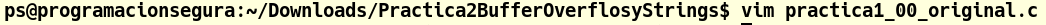
\includegraphics[width=1\textwidth]{mainmatter/Fotos Codigo/1.png}
 \\\\
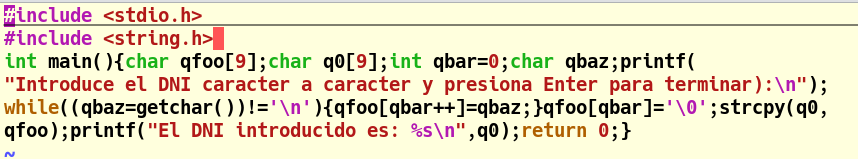
\includegraphics[width=1\textwidth]{mainmatter/Fotos Codigo/codigo sin indent.png}
\\\\
\noindent Podemos observer que el código no está totalmente ordenado, por lo tanto emplearemos el comando Indent para evitar errores y hacer de forma automática el indentado del código.
\\\\
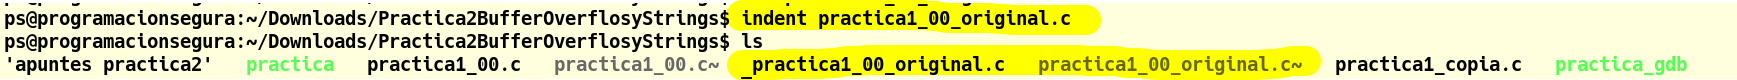
\includegraphics[width=1\textwidth]{mainmatter/Fotos Codigo/indent1.png}

\newpage 
\noindent Abrimos el código de nuevo y podemos ver que ya está correctamente formateado.
%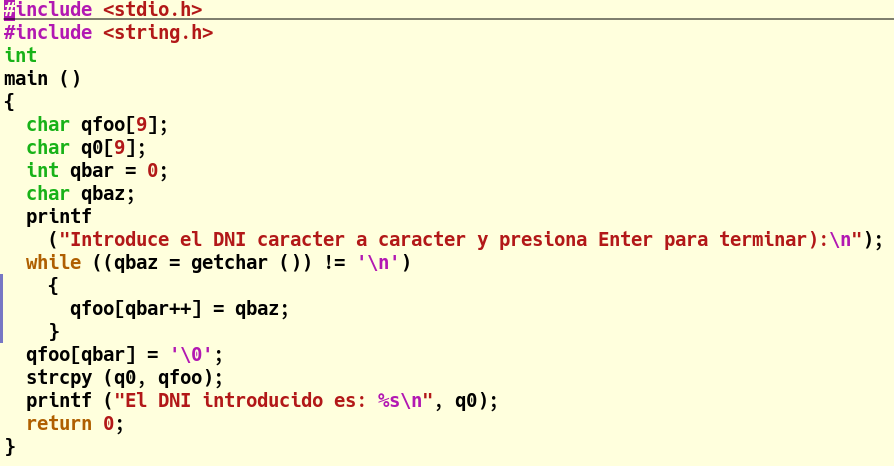
\includegraphics[width=1\textwidth]{mainmatter/Fotos Codigo/codigo formateado.png}
\\
\noindent Podemos ahora observar un fragmento de código en C que al parecer lee un DNI caracter a caracter, almacenándolo, y tras leer lo vuelve a imprimir.
\begin{verbatim}
#include <stdio.h>
#include <string.h>
int
main ()
{
  char qfoo[9]; //reservamos 9 caracteres en qfoo
  char q0[9]; //reservamos 9 caracteres en q0
  int qbar = 0; //inicializamos qbar a 0
  char qbaz;  //creamos variable qbaz de tipo caracter
  printf
    ("Introduce el DNI caracter a caracter y presiona 
    Enter para terminar):\n");
  while ((qbaz = getchar ()) != '\n') 
    //en qbaz guardamos lo que leemos y entramos al bucle            //mientras sea distinto de salto de línea
    {
      qfoo[qbar++] = qbaz; 
      //guardamos en cada iteración del while (donde qbar              //incrementa++), el caracter leído qbaz dentro de qfoo
    }
  qfoo[qbar] = '\0'; //ponemos el caracter nulo en la 
  //ultima posicion de qfoo (qbar)
  strcpy (q0, qfoo);  //hacemos strcpy de qfoo a q0, para                  //imprimir luego q0. OJO! STRCPY es insegura...
  printf ("El DNI introducido es: %s\n", q0);
  return 0;
}
\end{verbatim}

\noindent Primero crea un array qfoo de 9 caracteres,  q0[9], que es similar a qfoo y se crea un entero qbar inicializado en 0.
\\Ahora tras incializar los datos necesarios, el código imprime el mensaje que pide que se introduzca el DNI, y dentro del while se accederá a qfoo usando qbar como indice aumentando este uno a uno para así moverse dentro de qfoo. Asignará en cada posición el valor de qbaz, que es el caracter introducido en cada interación del bucle.
\\Ya por último se introduce el carácter nulo en qfoo y se usa strcpy para copiar el string de qfoo a q0, y se imprime q0 por pantalla.


\newpage
\section{Proceso de detección del problema}
\noindent Para detectar el problema vamos a ver si el problema "parece" hacer lo que debe:
\\Compilamos y ejecutamos: \\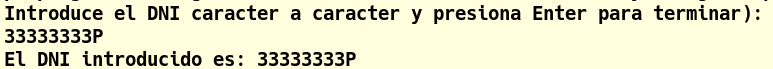
\includegraphics[width=1\textwidth]{mainmatter/Fotos Codigo/simple vista.png}
A simple vista, parece que el programa funciona correctamente, pero debemos tener en cuenta que cuando un programa entra para buscar problemas con él, ha pasado ciertas pruebas, por lo tanto, es normal que "aparentemente" funcione correctamemte. Vamos entonces a adentrarnos en materia y analizar el programa usando \textbf{Valgrind}.
\\
\vspace{0.3cm}
\noindent Primero compilamos el programa de nuevo pero con el flag -g para obtener trazas de debugging y poder usar valgrind.
\\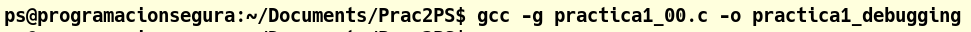
\includegraphics[width=1\textwidth]{mainmatter/Fotos Codigo/captura compilar debugging.png}
\\
Ejecutamos ahora el programa con valgrind...
\\
\textbf{El DNI introducido es: 888888888 }

==5378== HEAP SUMMARY: 
\\
==5378==     in use at exit: 0 bytes in 0 blocks 
\\
==5378==   total heap usage: 2 allocs, 2 frees, 2,048 bytes allocated 
\\
==5378== All heap blocks were freed -- no leaks are possible 
\\
==5378== ERROR SUMMARY: 1 errors from 1 contexts (suppressed: 0 from 0) 
\\
==5378== 1 errors in context 1 of 1: 
\\
==5378== Source and destination overlap in strcpy(0x1ffefffdd9, 0x1ffefffde2) 
\\
==5378==    at 0x484696F: strcpy (vg\_replace\_strmem.c:553) 
\\
==5378==    by 0x1091C6: main (practica1\_00.c:18) 
\\
\textbf{==5378== ERROR SUMMARY: 1 errors from 1 contexts (suppressed: 0 from 0)}
\vspace{0.3cm}
\\
\noindent Podemos observar como al introducir 9 caracteres el programa da error, mientras que si introducimos 8 caracteres no lo dará, por lo tanto se ha producido un buffer overflow.
\vspace{0.3cm}
\\
\textbf{El DNI introducido es: 8888888V }
\\
==5382== HEAP SUMMARY: 
\\
==5382==     in use at exit: 0 bytes in 0 blocks 
\\
==5382==   total heap usage: 2 allocs, 2 frees, 2,048 bytes allocated 
\\
==5382== All heap blocks were freed -- no leaks are possible 
\\
\textbf{==5382== ERROR SUMMARY: 0 errors from 0 contexts (suppressed: 0 from 0)}
\\
Los array qfoo y \verb|q0| están diseñados para almacenar un máximo de 9 caracteres. Sin embargo, cuando introduces un DNI de 9 dígitos, no queda espacio para el carácter nulo (\verb|\0|) que indica el final de una cadena en C. Al intentar copiar el contenido de \verb|qfoo| a \verb|q0| usando \verb|strcpy|, se produce un desbordamiento porque se intenta copiar un carácter más del que cabe en \verb|q0|.
\vspace{0.3cm}
\\
\textbf{¿Por qué no ocurre el error con 8 caracteres?}
\\
Cuando introduces 8 caracteres, el carácter nulo se almacena en la novena posición del arreglo, dejando espacio suficiente para ambos. Al utilizar \verb|strcpy|, se copia correctamente la cadena a \verb|q0| sin causar un desbordamiento.
\\
\newpage
\noindent Ahora vamos a hacer uso de la herramienta gdb para ver cómo se produce este buffer overflow:
\begin{verbatim}
ps@programacionsegura:$ gdb ./practica1\_debugging
(gdb) b 10 
Breakpoint 1 at 0x11b4: file practica1\_00\_original.c, line 17. 
(gdb) b 18 
Breakpoint 2 at 0x11c7: file practica1\_00\_original.c, line 18.
\end{verbatim}
\noindent Antes de causar el buffer overflow, vamos a ver dónde se escribe en memoria:
\begin{verbatim}
(gdb) x/64wx \$rsp 
0x7fffffffde40: 0x00000000 0x00000000 0x00000000 0x00000000 
0x7fffffffde50: 0x00000000 0x00000000 0x00000000 0x00000000 
0x7fffffffde60: 0x00000001 0x00000000 0xf7de424a 0x00007fff 

\end{verbatim}
\noindent Ahora cuando introducimos datos
\begin{verbatim}
Breakpoint 1, main () at practica1\_00\_original.c:17 
17        \textbf{strcpy} (q0, qfoo); 
(gdb) x/10wx \$rsp 
0x7fffffffde40: 0x00000000 0x00000000 0x00000000 0x00000000 
0x7fffffffde50: 0x39390000 0x39393939 0x0a003939 0x00000008 
    
\end{verbatim}
\noindent Saltamos a la linea 18 donde se hace strcpy...

\begin{verbatim}
Breakpoint 3, main () at practica1\_00\_original.c:18 
18   \textbf{printf} ("El DNI introducido es:, q0); 

(gdb) print qfoo 
\$2 = "99999999" OBSERVAMOS EL VALOR EN QFOO TRAS EL STRCPY

(gdb) x/64wx \$rsp 

0x7fffffffde40: 0x00000000 0x00000000 0x39393900 0x39393939 
0x7fffffffde50: 0x39390039 0x39393939 0x0a003939 0x00000008 
0x7fffffffde60: 0x00000001 0x00000000 0xf7de424a 0x00007fff 
 
\end{verbatim}
\noindent Si comparamos, podemos ver las posiciones de memoria en qfoo, pero ahora vamos a hacerlo pasándonos de datos a ver que ocurre:

\begin{verbatim}
Introduce el DNI caracter a caracter y presiona Enter para terminar): 
999999999999999999999999
99999999999999999999
99999999999999999999999999 

Breakpoint 1, main () at practica1\_00\_original.c:17 

17  \textbf{strcpy} (q0, qfoo); 

(gdb) x/10wx \$rsp 

0x7fffffffde40: 0x00000000 0x00000000 0x00000000 0x00000000 
0x7fffffffde50: 0x39390000 0x39393939 0x0a393939 0x00000074 
0x7fffffffde60: 0x00000001      0x00000000

\end{verbatim}

\noindent Aqui lo podemos observar antes del copy...

\begin{verbatim}
(gdb) x/10wx \$rsp 

0x7fffffffde40: 0x00000000 0x00000000 0x39393900 0x39393939 
0x7fffffffde50: 0x740a3939 0x39393900  0x0a393939 0x00000074 
0x7fffffffde60: 0x00000001 0x00000000 

(gdb) print qfoo 

\$1 = "\nt\n000999999"

\end{verbatim}
\noindent Podemos observar como lo que se encuentra en memoria ya comienza a fluctuar respecto de lo que deberíamos de ver si no hubiera problemas.
\newpage
\section{Ubicación y explicación del problema}
\noindent Ahora vamos a analizar el código para ver dónde se produce este buffer overflow. Como hemos visto al inicio del programa, se han reservado 9 posiciones en memoria para almacenar el string, pero claro, un DNI ocupa 9 posiciones, por lo tanto no se ha tenido en cuenta el carácter nulo,  que \verb|strcpy| usa para determinar el final de la cadena.
\vspace{0.3cm}
\\
\noindent Vamos a explicar los pasos que han llevado a este desbordamiento:
\begin{enumerate}
    \item \textbf{Almacenamiento del DNI en qfoo}
    \item \textbf{Uso de strcpy} / \textbf{no controlar el límite de lo que se lee}
    \item \textbf{Sobrescritura en memoria}
\end{enumerate}
Vamos a observar el array antes y después de usar strcpy:
\\
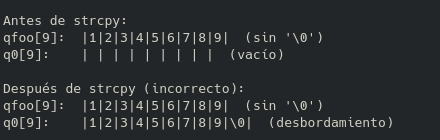
\includegraphics[width=0.75\textwidth]{mainmatter/Fotos Codigo/imagenantesdespuesstrcpy.png} 
\\
\section{Impacto del desbordamiento en la ejecución del programa}
\noindent Aunque el programa pueda seguir ejecutándose después de un desbordamiento de búfer, es fundamental comprender que esto no significa que el programa esté funcionando correctamente. Los efectos del desbordamiento pueden ser impredecibles y difíciles de detectar, pero siempre representan una amenaza para la seguridad y la estabilidad del programa.
\\
\newline Esto se debe básicamente a que en este programa, como es sencillo, no llegamos a hacer más cosas que imprimir únicamente el dni que hemos introducido, por lo tanto no hay mucha posibilidad de que este buffer overflow afecte al funcionamiento simple del programa.
\\
\newline 
Introduce el DNI caracter a caracter y presiona Enter para terminar): 
\\
999999999999999999999999999999999999999999999999999999999999999999999999999999999
\\999999999999999999999999999999999999999999999999999999999999999999999999999999999
\\999999999999999999999999999999999999999999999999999999999999999999999999999999999
\\999999999999999999999999999999999999999999999999999999999999999999999999999999...
\\
==6007== Source and destination overlap in strcpy(0x1ffefffdd9, 0x1ffefffde2) 
\\
==6007==    at 0x484696F: strcpy (vg\_replace\_strmem.c:553) 
\\
==6007==    by 0x1091C6: main (practica1\_00.c:18) 
\\
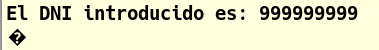
\includegraphics[width=0.5\textwidth]{mainmatter/Fotos Codigo/imagenimagem.png}
